\documentclass[11pt]{standalone}

\usepackage{garamondx}
\usepackage{pgfplots}
\usepackage{tikz}
\usepgfplotslibrary{units}
\usepackage{xcolor}
\definecolor{redtea}{rgb}{0.6823529412,0.2792156863,0.2666666667}
\usepackage{siunitx}
\usepackage{changepage}
\usepackage{calc}
\pgfplotsset{samples}
\usetikzlibrary{arrows,shapes,snakes,automata,backgrounds,petri,positioning}

\pgfdeclarelayer{background}
\pgfdeclarelayer{foreground}
\pgfsetlayers{background,main,foreground}

\usetikzlibrary{arrows,shapes,snakes,automata,backgrounds,petri}
\usetikzlibrary{calc}
\tikzset{stretch/.initial=1}
\newcommand\drawloop[4][]%
{\draw[shorten <=0pt, shorten >=0pt,#1]
	($(#2)!\pgfkeysvalueof{/tikz/stretch}!(#2.#3)$)
	let \p1=($(#2.center)!\pgfkeysvalueof{/tikz/stretch}!(#2.north)-(#2)$),
	\n1= {veclen(\x1,\y1)*sin(0.5*(#4-#3))/sin(0.5*(180-#4+#3))}
	in arc [start angle={#3-90}, end angle={#4+90}, radius=\n1]%
}

\usepackage{pgfplots}
\usepgfplotslibrary{polar}
\pgfplotsset{compat=newest}

\begin{document}
	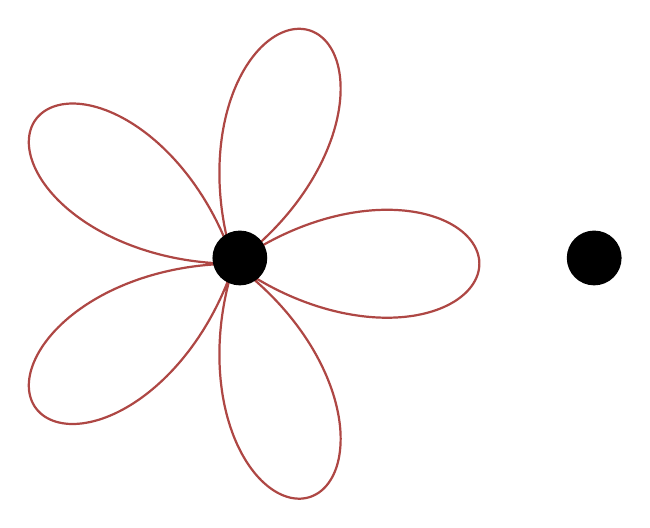
\begin{tikzpicture}[node distance=1.7cm,shorten <=.4ex, shorten >=.4ex,>=latex]
	\coordinate[] (n0) at (3.5,3.5);
	\coordinate[] (n1) at (8,3.5);
	\coordinate[] (n2) at (1,0);
	\coordinate[] (n3) at (0,-1);
	\coordinate[] (n4) at (-1,0);
	\coordinate[] (n5) at (-2,0);
	\coordinate[] (n6) at (2,0);
	
	\begin{polaraxis}[grid=none, axis lines=none,redtea]
	\addplot[mark=none,domain=0:370,samples=300,smooth,thick] {abs(cos(5*x/2))};
	\end{polaraxis}
	%\draw[redtea] (n0.90) arc (0:264:4mm);
	%\draw[thick,->,shorten >=1pt] (n0) to [out=90,in=180,loop,looseness=4.8] (n0);
	%\draw[thick,->] (n0) to [out=90,in=180,looseness=5] (n0);
	%\draw [] (n0.east) -- (n0.west);
	
	\node at (n0)[circle,fill,inner sep=0.7em]{};
	\node at (n1)[circle,fill,inner sep=0.7em]{};
	


	
	%\draw[->,>=latex,redtea,shorten >=5pt]([xshift=3pt,yshift=0pt]a)--([xshift=3pt,yshift=0pt]b);
	%\draw[->,>=latex,redtea,shorten >=5pt]([xshift=0pt,yshift=0pt]a)--([xshift=0pt,yshift=0pt]a);
	\end{tikzpicture}
\end{document}
